
\documentclass[a4paper]{article}

\usepackage{graphicx}
\usepackage{listings}
\usepackage{indentfirst}
\usepackage{float}
%\usepackage[T1]{fontenc}                % F�r svenska bokst�ver
%\usepackage[swedish]{babel}             % F�r svensk avstavning och svenska
                                        % rubriker (t ex "inneh�llsf�rteckning)
\title{Programming Project, Database Technology}
\author{Tim Dolck dat11tdo@student.lu.se \\ 
Julian Kron� dat11jkr@student.lu.se \\
Christopher Nilsson dat11cni@student.lu.se \\
Computer science, LTH}
%\date{}           % Blir dagens datum om det utel�mnas

\begin{document}
\lstset{language=SQL}

\maketitle
\newpage
\section{Introduction}
\section{Requirements}
\section{Outline}
\section{Model}

\subsection{E/R Diagram}

An overview of the database design can be seen in figure~\ref{model}.

\begin{figure}[H]
  \centering
  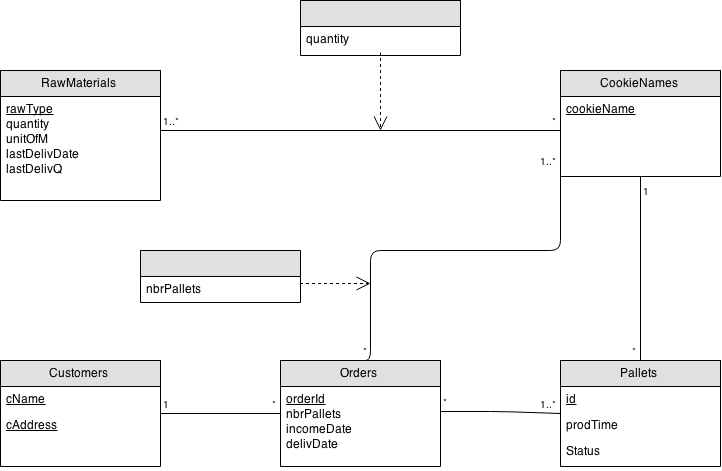
\includegraphics[width=\textwidth]{cookies.png}
  \caption{An UML diagram illustrating the database design.}
  \label{model}
\end{figure}

\subsection{Relations}
\section{Statements}
\end{document}                 % The input file ends with this command.
